\documentclass[a4paper,11pt]{article}

\usepackage{fullpage}
\usepackage[french]{babel}

\usepackage[utf8]{inputenc}
\usepackage[T1]{fontenc}

% These fonts do not work on my computer, you can change this if you feel like it
% Font : (better idea ?)
%\usepackage{newpxtext} 
%\usepackage{newpxmath}
\usepackage{mathpazo}

\usepackage{url}
%for images
\usepackage{graphicx}
%for code-quoting
\usepackage{listings}
%for pseudo-code algo
\usepackage{algorithm}
\usepackage{algpseudocode}
% Parameters for listings

\lstset{%
  basicstyle=\footnotesize\sffamily,%
  columns=fullflexible,%
  frame=lb,%
  frameround=fftf,%
  language=caml,%
}%

\begin{document}

\begin{titlepage}
  \title{Tours de Hanoï et Pavage de Penrose}
  \author{Guillaume Barbier, Romain Ferrand}
  \date{\today}

  \maketitle

  \begin{abstract}
    
  \end{abstract}
\end{titlepage}

\section*{Introduction}
  Dans ce document nous allons vous présenter notre étude des tours de Hanoï et du
  pavage de Penrose. Nous avons proposé des algorithmes répondant aux problèmes posés, puis
  nous avons proposé certaines améliorations à ces algorithmes, en terme de contraintes posées,
  de structure de donnée ou encore d'affichage.

\section{Pavage de Penrose}
\label{chap:penrose}



\subsection{Présentation du problème}
\label{sec:prezPenrose}
\begin{figure}
  \centering
  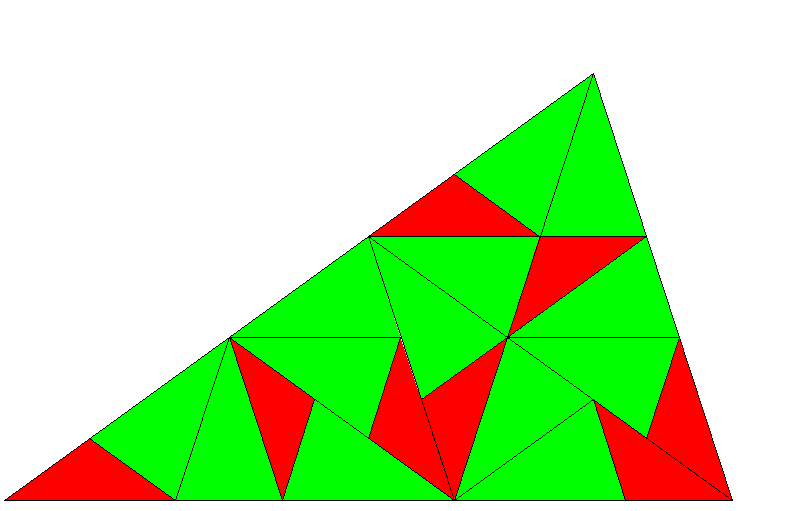
\includegraphics[width=0.8\textwidth]{penrose_example.png}
  \caption{Pavage de Penrose à trois générations}
  \label{fig:penrose_example}
\end{figure}

Le pavage de Penrose est un pavage du plan non périodique découvert par le mathématicien
britannique Roger Penrose dans les années 1970.
Notre but sera de découper un triangle d'or (dont les côtés ont un ratio égal au nombre d'or)
en des triangles de même forme selon les règles suivantes,
et de répéter cette action sur les triangles ainsi formés.

\begin{figure}
  \centering
  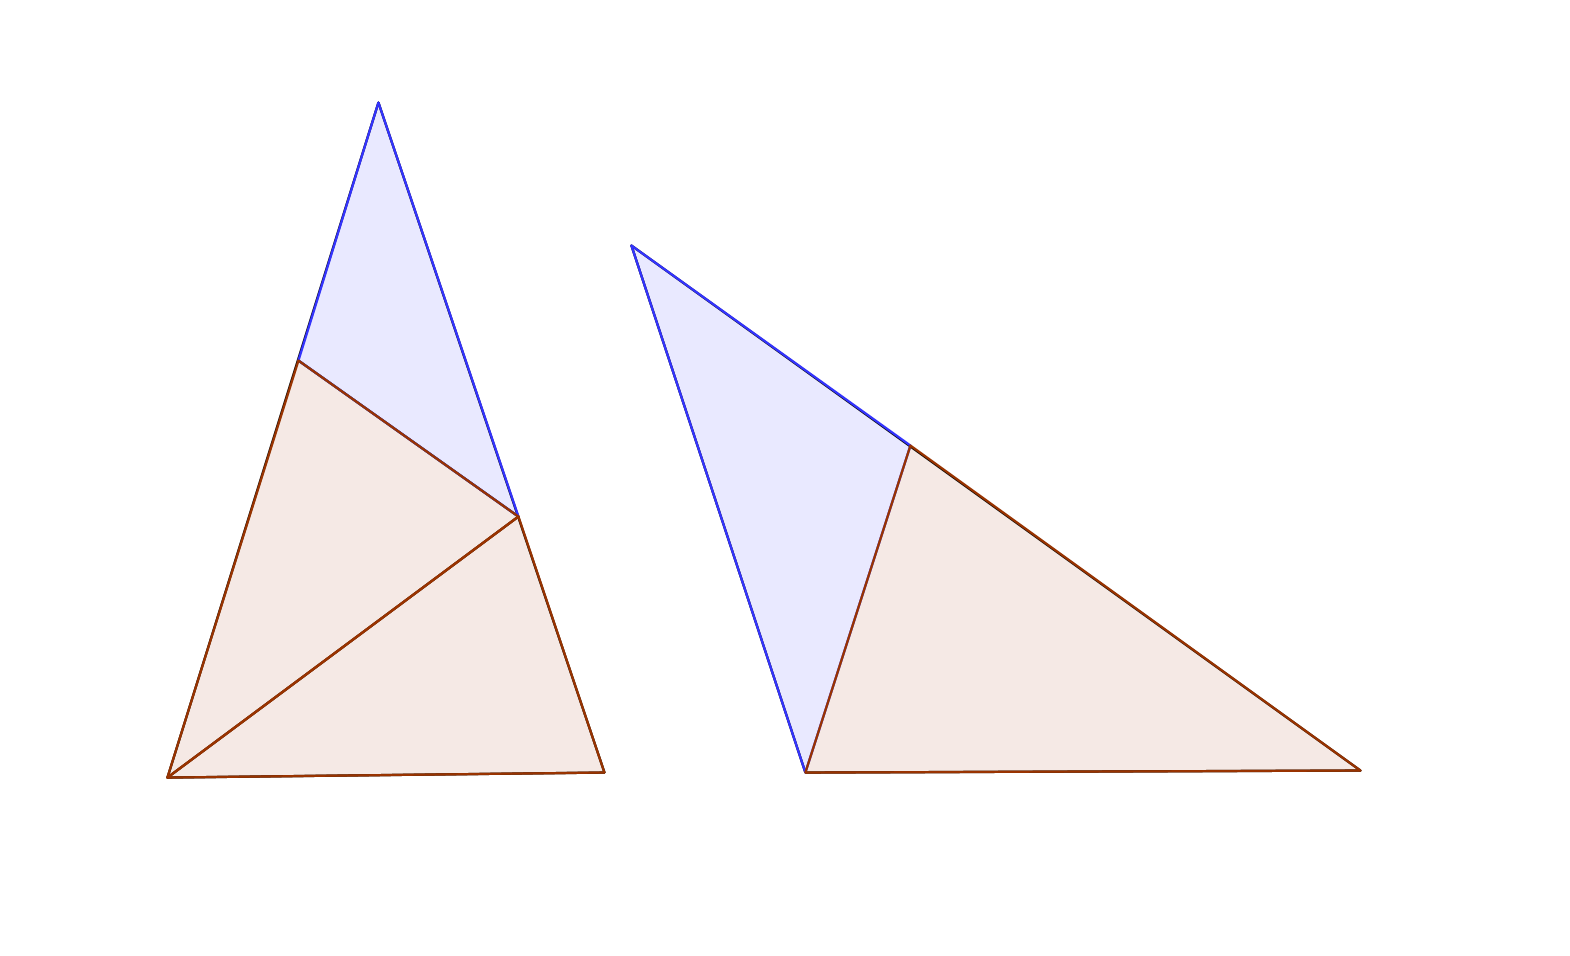
\includegraphics[width=0.8\textwidth]{division_penrose.png}
  \caption{Division des deux types de triangle}
  \label{fig:penrose_example}
\end{figure}

\subsubsection{Première implémentation}
\label{sec:algoBasePenrose}
On cherche à découper un triangle d'or un certain nombre de fois. Chaque découpage successif
forme une nouvelle \og génération \fg de triangles. Cette succession de génération forme
un arbre dans lequel chaque nœud et feuille représente un triangle. Pour afficher la
$n$-ième génération, il suffit de dessiner les nœuds de profondeur $n$.\\

L'algorithme le plus simple se résume ainsi :

\begin{itemize}
  \item On parcourt l'arbre des triangles (dans un ordre quelconque).
  \item À chaque feuille, on dessine le triangle associé.\\
\end{itemize}

L'intérêt de cette méthode est qu'elle peut être rendue polymorphe. Il n'est pas nécessaire
de parler de triangle, on peut parler de polygone, voire même de forme ou d'objet.
Pour celà, il faut fournir à l'algorithme:

\begin{itemize}
  \item un objet initial à découper qui sert de racine à l'arbre;
  \item une fonction pour diviser un objet père en ses objets fils;
  \item une fonction pour dessiner un objet (en particulier les feuilles).\\
\end{itemize}

On définit donc un type $triangle$, et les fonctions définies ci-dessus. Cependant,
je préfère m'attarder sur l'algorithme lui même plutôt que sur la façon dont on affiche
et divise les triangles.

\subsection{Comment améliorer l'algorithme ?}

\subsubsection{Le dessin des contours}
\begin{figure}
  \centering
  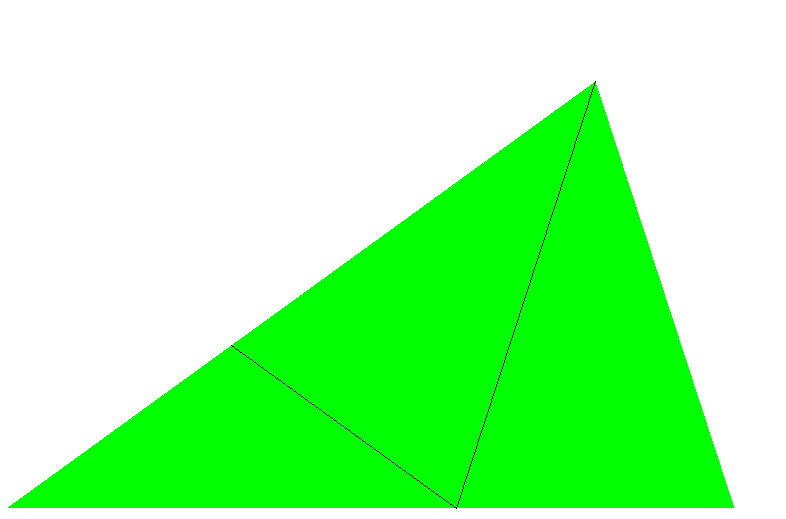
\includegraphics[width=0.8\textwidth]{penrose_inline1.png}
  \caption{Séparation des triangles fils}
  \label{fig:penrose_example}
\end{figure}
Nous dessinons les triangles avec leur contour, cependant le côté d'un triangle est souvent
un côté du triangle voisin, ou une section d'un côté du triangle parent.\\

Comment alors modifier notre algorithme pour dessiner chaque trait une unique fois ?\\

Il faut changer de point de vue : un trait ne permet pas seulement de dessiner le contour
d'un triangle, mais de séparer deux triangles. Ainsi nous allons pouvoir dessiner à chaque fois
que l'on divise un triangle (c'est à dire à chaque nœud), pour séparer
les triangles nouvellement formés.\\

Lorsque deux triangles sont côte à côte, ils seront alors séparés par un trait dessiné
par le nœud qui est leur plus proche ancêtre commun. Cependant le contour du triangle racine
n'est pas pris en compte par cette méthode, il faut donc penser à le dessiner.\\

L'algorithme devient alors:
\begin{itemize}
  \item On dessine le contour de l'objet racine.
  \item On parcours l'arbre dans un ordre quelconque.
  \item À chaque nœud, on dessine les séparations entre les fils de ce nœud.
  \item À chaque feuille, on dessine l'objet associé.\\
\end{itemize}

L'algorithme a besoin de :
\begin{itemize}
  \item un objet initial à découper qui sert de racine à l'arbre;
  \item une fonction pour diviser un objet père en ses objets fils;
  \item une fonction pour dessiner un objet (en particulier les feuilles);
  \item une fonction pour dessiner les séparations entre les fils d'un objet.
\end{itemize}

\subsubsection{Le dessin des générations successives}
On cherche maintenant à dessiner successivement plusieur générations. Chaque génération
correspond à une hauteur particulière dans notre arbre, nous allons donc naturellement
utiliser un parcours en largeur de l'arbre. Cependant, nous avons aussi besoin de nous
arrêter avant chaque génération pour pouvoir effectuer le dessin.\\

Pour cela, la fonction récursive de parcours en largeur prendra en paramètre la liste des
nœuds d'une certaine hauteur (la génération en cours de traitement) privé des nœuds déjà
traités; la liste des nœuds de la génération suivante, qui est vide au premier appel sur
cette génération mais qui se remplie au fil des appels récursifs.\\

Cela n'est pas tout, il faut aussi prendre en compte le dessin des séparateurs. Dans
l'algorithme précédent, nous nous contentions de dessiner les séparations au niveau de chaque
nœud lors de l'unique parcours de l'arbre. Ici, lors du dessin de chaque génération, il
faut reparcourir les générations précédentes pour dessiner les séparateurs au niveau de
chaque nœuds. Comme la division des objets peut être couteuse (dans le cas des triangles, elle
ne l'était pas), nous avons décidé de stocker les nœuds déjà parcourus dans une liste.\\

L'algorithme est schématiquement :

\begin{lstlisting}
  let rec parcours_largeur generation generation_suivante n =
    if n = 0 then
      ()
    else if est_vide generation then begin
      (*On a fini de parcourir cette generation *)
      dessiner_separateurs liste_des_noeuds_deja_visites;
      dessiner_generation generation_suivante;
      parcours_largeur generation_suivante vide (n-1)
    end else begin
      let noeud = extraire_noeud generation
      and suite = extraire_suite generation
      in
      let generation_suivante = concatenation (obtenir_fils noeud) generation_suivante
      in
      ajouter_noeud liste_des_noeuds_deja_visites noeud;
      parcours_largeur suite generation_suivante n
    end
  ;;
\end{lstlisting}
Pour gérer les arguments contenant les générations, nous avions le choix entre des listes et
des files, cependant ces deux implémentations donnent un même coût en mémoire et en espace,
nous avons donc choisi d'utiliser des listes car nous avons plus l'habitude d'utiliser ces
objets.\\

\subsection{Conclusion}
Nous avons réussi à créer un algorithme efficace qui répond aux contraintes que nous nous
sommes posés. Cependant, cet algorithme parcours l'arbre de nombreuses fois car il doit
afficher les séparateurs à chaque nœud à chaque affichage. Le gain était de ne pas avoir
à afficher plusieurs fois le même trait, mais on peut se demander si cela est réellement pire
que de reparcourir l'arbre.
\end{document}